\indent Skomprimovaný balík obsahuje zdrojový kód k webstránke, serveru, aj k aplikácii Passer (rozdelené do priečinkov). Na otestovanie celého riešenia je nutné nainštalovať Passer na zariadenie iPhone 5S a vyššie.

Po rozbalení balíka, v priečinku \textit{iOS - Passer App} sa nachádza súbor \textit{Passer.xcodeproj}. Pred otvorením tohto súboru je potrebné:
\begin{itemize}
    \item[-] Mať nainštalovaný operačný systém macOS Catalina, alebo vyššie
    \item[-] Mať nainštalované prostredie Xcode a jeho najnovšiu verziu
\end{itemize}

\noindent Teraz môžeme otvoriť \textit{Passer.xcodeproj}. Po otvorení je v hornom paneli jeden warning (ikona so žltým výkričníkom):

\begin{figure}[H]
  \centering
  
\includegraphics[width=14cm]{img/tutorial1.png}
  \label{tutorial1}
\end{figure}

\noindent Po kliknutí na ikonu napravo sa warning zobrazí v ľavom paneli, ako vidno na nasledujúcom obrázku: 

\begin{figure}[H]
  \centering
  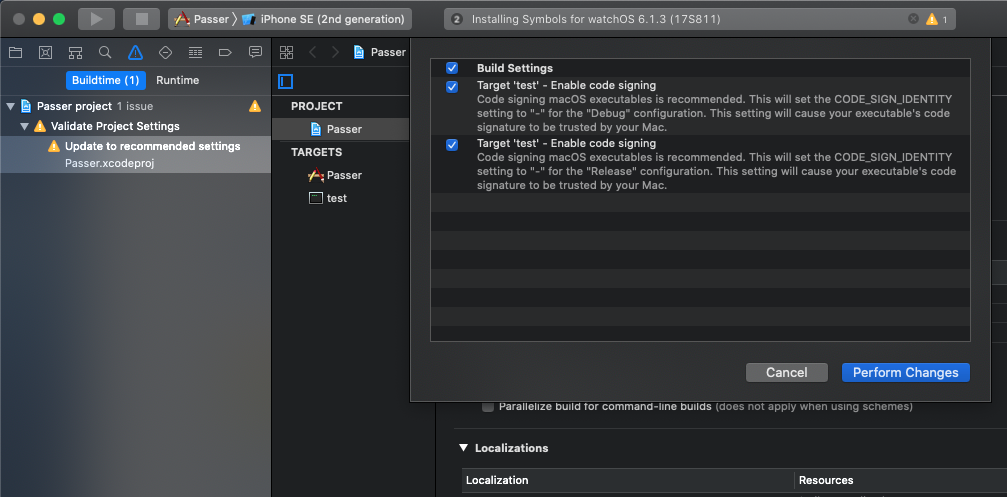
\includegraphics[width=15cm]{img/tutorial2.png}
  \label{tutorial2}
\end{figure}

\noindent Klikneme na ,,Update to recommended settings'' a v okne, ktoré sa následne zobrazí klikneme na ,,Perform Changes''.

Následne si potrebujeme v Xcode nastaviť AppleID. V \textit{Xcode --> Preferences...}, v sekcii \textit{Accounts}, vľavo dole klikneme na ,,+'' a prihlásime sa do Apple ID (\textbf{musí mať aktivovaný free developer program. Viac na https://developer.apple.com/}).

\begin{figure}[H]
  \centering
  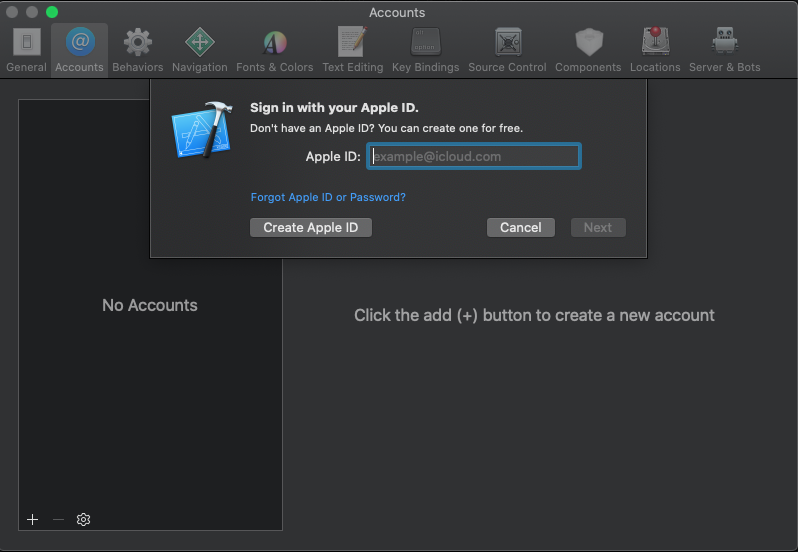
\includegraphics[width=14cm]{img/tutorial3.png}
  \label{tutorial3}
\end{figure}

\noindent Po pridaní Apple ID do Xcode, vyzerá sekcia \textit{Accounts} v \textit{Preferences...} takto:

\begin{figure}[H]
  \centering
  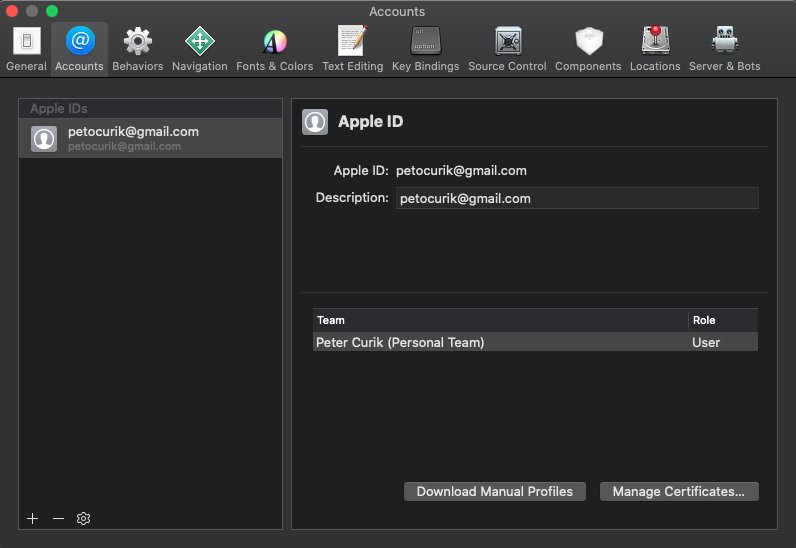
\includegraphics[width=14cm]{img/tutorial4.png}
  \label{tutorial4}
\end{figure}

\noindent Zatvoríme okno s nastaveniami. Do Macu pripojíme iPhone pomocou lightning kábla.
\newpage

\begin{figure}[H]
  \centering
  
\includegraphics[width=10cm]{img/tutorial5.png}
  \label{tutorial5}
\end{figure}

\noindent Vľavo hore v Xcode vidíme tlačidlo (prvé sprava), ktorým vieme určiť, na akom zariadení sa má skompilovať program. Klikneme na neho a vyberieme úplne prvé zariadenie (fyzické zariadenie - pripojený iPhone do Macu):

\begin{figure}[H]
  \centering
  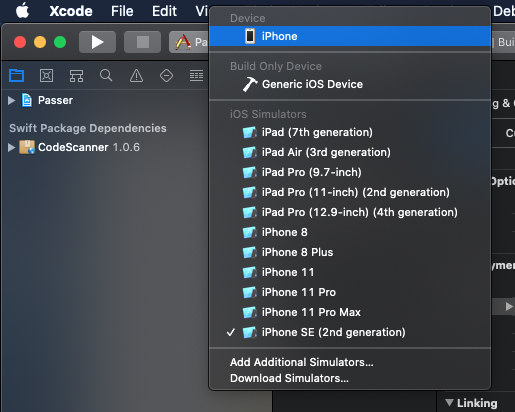
\includegraphics[width=14cm]{img/tutorial6.png}
  \label{tutorial6}
\end{figure}

Teraz môžeme spustiť program stlačením tlačidla vľavo hore, s ikonou bieleho trojuholníka (všobecne známe ako tlačidlo ,,play''). Pred spustením vyžaduje Xcode heslo, ktorým sa prihlasujeme do Macu.

\begin{figure}[H]
  \centering
  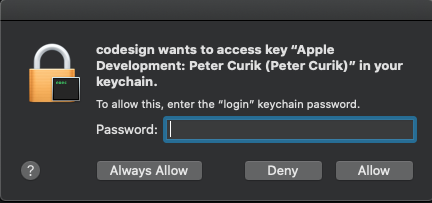
\includegraphics[width=10cm]{img/tutorial7.png}
  \label{tutorial7}
\end{figure}

Po zadaní hesla začína proces kompilovania aplikácie. Spustenie je neúspešné. Nasledovná hláška nás inštruuje, čo je nutné zmeniť v nastaveniach pripojeného iPhonu: 

\begin{figure}[H]
  \centering
  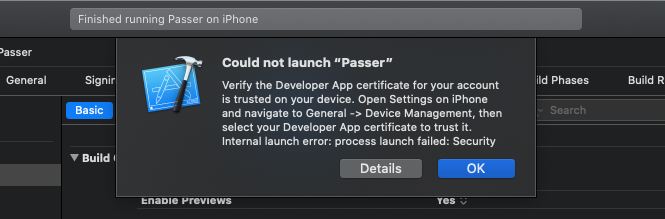
\includegraphics[width=13cm]{img/tutorial8.png}
  \label{tutorial8}
\end{figure}

\noindent Zmeníme povolenia v nastaveniach iPhonu podľa inštrukcií Xcode-u. V Xcode klikneme na ,,OK''. Následne aplikáciu skompilujeme znovu. Tentokrát úspešne. Môžeme používať Passer na danom iPhone zariadení. \newline

\textbf{Upozornenie:} Passer nie je optimalizovaný pre všetky iPhone zariadenia. Vývoj aplikácie bol testovaný iba na zariadení iPhone 7 Plus. Veľkosť písma bola v zariadení nastavená na najmenšiu. V prípade, že by sa na inom iPhone vyskytli chyby používateľského rozhrania, odporúčame aspoň nastaviť veľkosť textu na najmenšiu.

Passer nie je možné spúšťať pomocou iOS simulátorov. Keďže aplikácia využíva Secure Enclave, čo je separátny hardvér v telefóne, je nutné využívať výhradne fyzické zariadenie.